\section{Project Setup}

\subsection{Prerequisites}

The project is built with \textbf{CMake 4.1} and targets the \textbf{C11} language standard. Before building, the following tools must be present on the host machine:

\begin{itemize}
    \item \textbf{C compiler with C11 support} — either GCC (\texttt{gcc}) or Clang (\texttt{clang}) will work. The compiler must accept the \texttt{-std=c11} flag. GCC 5+ and Clang 3.3+ both satisfy this requirement.
    \item \textbf{CMake 4.1 or later} — used to generate the native build system files. CMake is platform-independent and produces Makefiles on Linux, Xcode project files on macOS, and Visual Studio solution files on Windows. Download from \texttt{cmake.org} or install via a package manager.
    \item \textbf{GNU Make} (Linux/macOS only) — required to consume the Makefile that CMake generates on Unix-like systems. On macOS, Make ships with the Xcode Command Line Tools (\texttt{xcode-select -{}-install}). On Windows, CMake targets MSBuild or Ninja instead, so Make is not needed.
\end{itemize}

Recommended development environments by platform:

\begin{itemize}
    \item \textbf{Windows} — Visual Studio 2022 (Community edition is free). CMake integrates natively and can target the MSVC toolchain or the bundled Clang front-end.
    \item \textbf{macOS / Linux} — JetBrains CLion, which has built-in CMake support and a bundled GDB/LLDB debugger. VS Code with the \textit{CMake Tools} and \textit{C/C++} extensions is a lightweight alternative.
\end{itemize}

\subsection{File Directory}

The repository is organised into three top-level directories: \texttt{src/} for all translation units, \texttt{include/} for their corresponding headers, and \texttt{docs/} for the \LaTeX{} paper. Source files are further grouped by responsibility:

\begin{figure}[H]
\centering
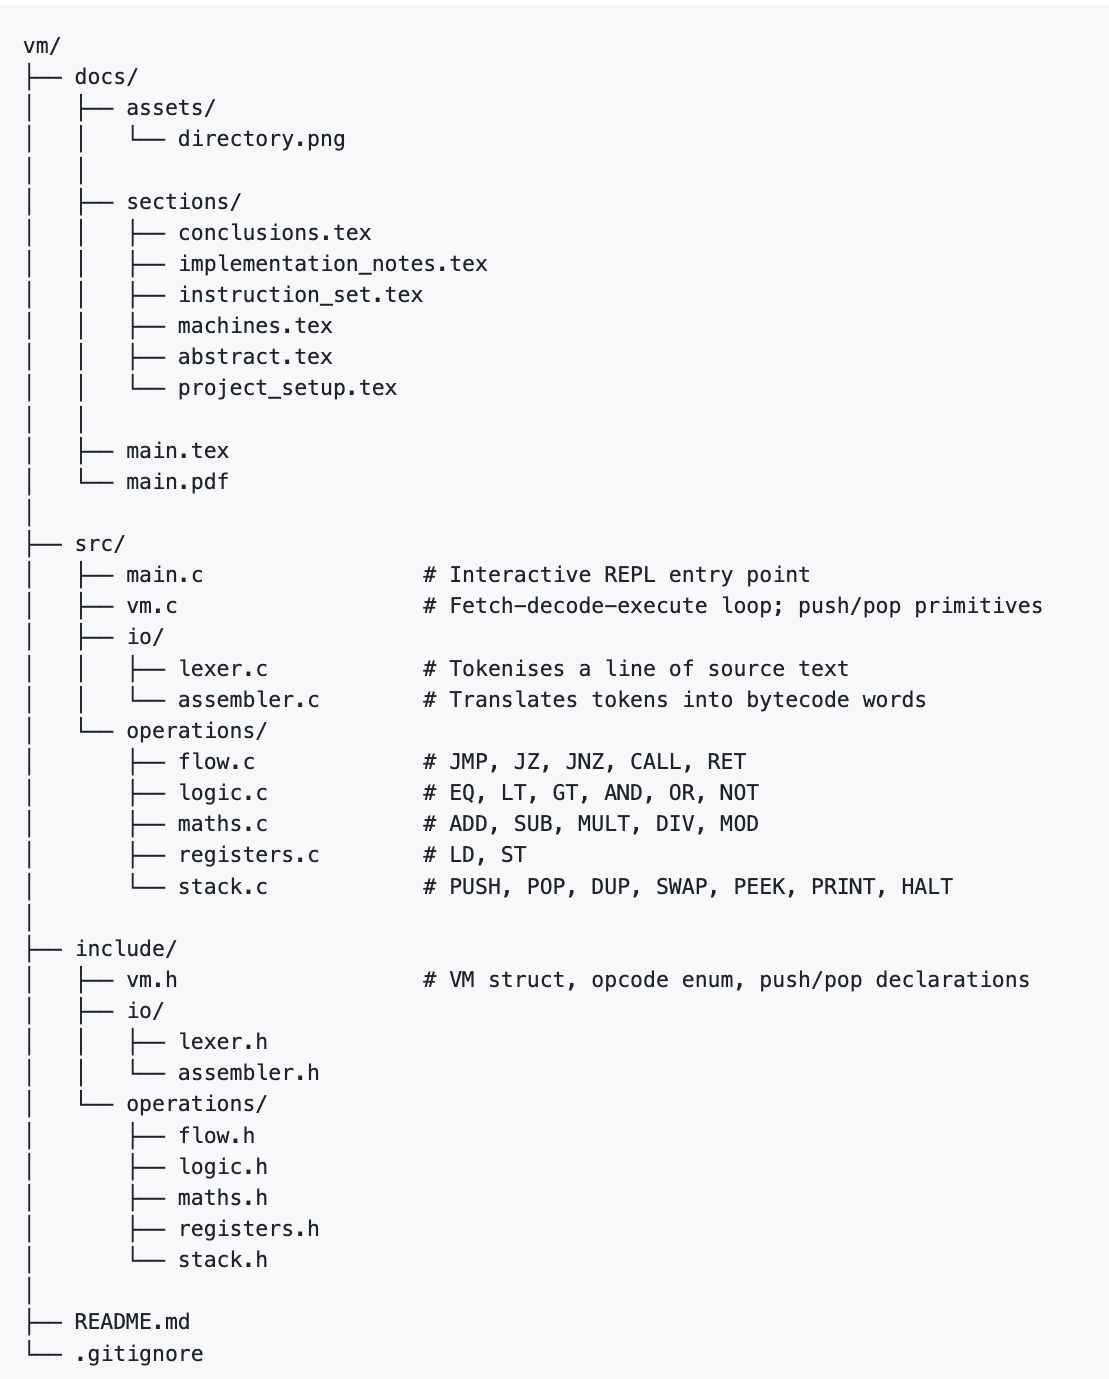
\includegraphics[width=0.8\textwidth]{assets/directory.png}
\caption{File Directory of the project}
\end{figure}

Every \texttt{.c} file under \texttt{src/operations/} is a self-contained translation unit. It includes only its own header and \texttt{vm.h}; it has no knowledge of sibling modules. This layout enforces at the filesystem level the same separation of concerns described in the architecture section.

\subsection{Build}

\subsubsection*{Option A — CMake (recommended)}

CMake is the canonical way to build the project. From the repository root:

\begin{lstlisting}[language=bash]
# 1. Create and enter a build directory
mkdir build && cd build

# 2. Configure (generates Makefile / solution)
cmake ..

# 3. Compile
cmake --build .
\end{lstlisting}

The resulting executable is placed at \texttt{build/virtual\_machine} on Unix-like systems and \texttt{build\textbackslash Debug\textbackslash virtual\_machine.exe} on Windows.

\subsubsection*{Option B — Direct GCC / Clang invocation}

For environments without CMake, the project can be compiled with a single command from the repository root:

\begin{lstlisting}[language=bash]
gcc -std=c11 -Wall -Wextra -Iinclude \
    src/main.c src/vm.c \
    src/io/lexer.c src/io/assembler.c \
    src/operations/maths.c src/operations/stack.c \
    src/operations/flow.c src/operations/logic.c \
    src/operations/registers.c \
    -o vm
\end{lstlisting}

Replace \texttt{gcc} with \texttt{clang} if that is the installed compiler. The flags \texttt{-Wall -Wextra} enable a broad set of compiler warnings; the project compiles cleanly at both levels.

\subsection{Running the VM}

Once compiled, launch the interactive assembler from the directory containing the binary:

\begin{lstlisting}[language=bash]
./vm          # Unix-like systems
vm.exe        # Windows
\end{lstlisting}

The REPL greets the user and waits for input. A brief example session — pushing two values, adding them, printing the result, and halting — looks like this:

\begin{lstlisting}
Virtual Machine -- interactive assembler
Type HELP for usage, QUIT to exit.

> PUSH 10
  [@ word 0]
> PUSH 32
  [@ word 2]
> ADD
  [@ word 4]
> PRINT
  [@ word 5]
> HALT
  [@ word 6]
>
--- Running (7 word(s)) ---
42
--- Done ---
\end{lstlisting}

The shell also accepts four meta-commands that are processed by the REPL and never assembled into the program:

\begin{center}
\begin{tabular}{ll}
\toprule
\textbf{Command} & \textbf{Effect} \\
\midrule
\texttt{RUN}   & Assemble and execute the current buffer \\
\texttt{LIST}  & Print each word with its bytecode index \\
\texttt{RESET} & Clear the program buffer \\
\texttt{HELP}  & Display the full opcode reference \\
\texttt{QUIT} / \texttt{EXIT} & Exit the program \\
\bottomrule
\end{tabular}
\end{center}

A blank line is equivalent to \texttt{RUN}. Lines beginning with \texttt{;} are treated as comments and stripped before lexing.

\subsection{Separation of Concerns}

The codebase is structured around a strict \textit{separation of concerns}: no module knows about the internals of another module it does not directly depend on. The dependency graph is deliberately shallow:

\begin{itemize}
    \item \textbf{Operation modules} (\texttt{maths}, \texttt{logic}, \texttt{flow}, \texttt{registers}, \texttt{stack}) depend only on \texttt{vm.h}. They are entirely unaware of one another.
    \item \textbf{\texttt{vm.c}} depends on all five operation headers, but only to dispatch via \texttt{case} labels. It contains no arithmetic or logic of its own.
    \item \textbf{\texttt{assembler.c}} depends on \texttt{vm.h} (for the opcode enum) and \texttt{lexer.h} (for the \texttt{Token} type). It knows nothing about runtime execution.
    \item \textbf{\texttt{lexer.c}} depends on nothing beyond the C standard library. It is the most isolated module in the project.
    \item \textbf{\texttt{main.c}} is the sole integration point, pulling together the lexer, assembler, and VM.
\end{itemize}

A practical consequence of this design: adding a new opcode requires changes to at most three files — the \texttt{enum} in \texttt{vm.h}, the relevant operation source file, and the mnemonic table in \texttt{assembler.c}. No other file needs to be touched, and the REPL automatically recognises the new instruction without any further modification.